\documentclass[UTF8,11pt,a4paper]{ctexart}
\usepackage[margin=22mm,headheight=15pt,includeheadfoot]{geometry}
\usepackage{graphicx,booktabs,tabularx,array,float,caption}
\usepackage[table]{xcolor}
\usepackage{enumitem,listings,tikz,fancyhdr,lastpage,hyperref,titlesec,amssymb}
\usetikzlibrary{arrows.meta,positioning,shapes.geometric}
\definecolor{Navy}{HTML}{17365D}\definecolor{Blue}{HTML}{2F75B5}\definecolor{Teal}{HTML}{2A9D8F}\definecolor{Sky}{HTML}{EAF3F8}\definecolor{Ink}{HTML}{263238}\definecolor{SoftGray}{HTML}{F4F6F8}
\hypersetup{colorlinks=true,linkcolor=Navy,urlcolor=Blue}
\graphicspath{{figures/}}
\captionsetup{font=small,labelfont=bf,labelsep=period,justification=centering}
\setlist{itemsep=0.25em,topsep=0.3em}\setlist[enumerate]{leftmargin=1.7em}
\setlength{\parindent}{2em}\setlength{\parskip}{0.28em}
\titleformat{\section}{\large\bfseries\color{Navy}}{\thesection}{0.6em}{}
\titleformat{\subsection}{\normalsize\bfseries\color{Blue}}{\thesubsection}{0.6em}{}
\pagestyle{fancy}\fancyhf{}\fancyhead[L]{\small 第17组 · 机器人学集成小组项目}\fancyhead[R]{\small 实验二：机械臂定点抓取}\fancyfoot[C]{\small 第 \thepage 页}\renewcommand{\headrulewidth}{0.35pt}\renewcommand{\footrulewidth}{0.35pt}
\lstset{basicstyle=\ttfamily\footnotesize,breaklines=true,columns=fullflexible,keepspaces=true,backgroundcolor=\color{SoftGray},frame=single,rulecolor=\color{Blue!35},xleftmargin=0.8em,xrightmargin=0.8em,aboveskip=0.5em,belowskip=0.6em}
\newcommand{\code}[1]{\texttt{\footnotesize #1}}\newcommand{\resultbox}[1]{\begin{center}\fcolorbox{Navy}{Sky}{\parbox{0.93\textwidth}{\small #1}}\end{center}}
\begin{document}
\begin{titlepage}\thispagestyle{empty}
\begin{tikzpicture}[remember picture,overlay]\fill[Navy] (current page.north west) rectangle ([yshift=-34mm]current page.north east);\fill[Teal] ([yshift=-34mm]current page.north west) rectangle ([yshift=-37mm]current page.north east);\end{tikzpicture}
\vspace*{12mm}\begin{flushright}\color{white}\small 机器人学集成小组项目\end{flushright}\vspace{18mm}
\begin{center}{\color{Navy}\fontsize{25}{30}\selectfont\bfseries 实验二\\[2mm]}{\color{Blue}\fontsize{19}{24}\selectfont 机械臂定点抓取与放置}\par\vspace{11mm}\rule{0.72\textwidth}{1pt}\par\vspace{5mm}{\large 实验报告}\par\vspace{8mm}
\begin{tabular}{>{\bfseries\color{Navy}}p{0.23\textwidth}p{0.58\textwidth}}课程 & 机器人学集成小组项目 I\\小组 & 第17组\\组员 & 杨牧青；兰松语；张凯睿；赵航\\平台 & ROS 2 Humble + Gazebo + mechArm 270\\材料版本 & experiment2\_submission\_final\_20260913\_v2\\仓库 & \url{https://github.com/9161942-boop/robotics-experiment-2}\end{tabular}
\vfill\begin{minipage}{0.78\textwidth}\small\color{Ink}本报告记录一个定点抓取与放置实验：目标物体预先放在 A 点，机械臂使用平行夹爪完成抓取，抬升到安全高度后移动到 B 点并释放，最后回到初始位姿。报告分别说明控制原理、ROS 2 实现、仿真验证结果以及实机演示证据。\end{minipage}\vfill{\color{Navy}\large 2026 年 9 月}\par\end{center}\end{titlepage}
\section*{摘要}\addcontentsline{toc}{section}{摘要}
本实验面向六关节 mechArm 270 机械臂，完成了一个可重复的定点抓取与放置任务。系统采用 ROS 2 工作空间组织，通过一个 Launch 文件同时启动机器人描述、Gazebo 场景、控制器、状态发布、可视化节点和任务节点。预设动作序列使机械臂从 home 位姿运动到抓取点 A，闭合夹爪并抬起圆柱目标，随后移动到放置点 B，通过短距离竖直下降释放目标，最后返回 home。任务节点在关节空间中使用余弦插值，在每个阶段发布状态和结果信息，检查关节限位，并将状态转移记录到 CSV。最终 v2 材料中的两份独立五周期记录均包含 5 条\code{cycle\_passed}，终端摘要为\code{status: passed}且\code{success\_count=5}。仿真视频记录 Gazebo 中的完整动作，实机视频记录实体机械臂的操作过程；两类材料共同构成实验取证。\par
\noindent\textbf{关键词：} ROS 2；Gazebo；mechArm 270；定点操作；夹爪控制；实验报告

\section{实验目的与验收要求}
\subsection{实验目的}
本实验搭建并说明一条完整的机械臂操作流程。机械臂回到已知 home 位姿，沿安全路径接近目标，完成夹爪闭合和打开，并将目标从固定抓取点 A 转移到固定放置点 B。A、B 点在参数文件中预先给出，实验评价动作顺序、控制稳定性和结果可重复性。

实验先在 Gazebo 中验证机器人模型和控制器，再将相同的 ROS 2 控制语义迁移到实体 mechArm 270。迁移阶段更新设备通信、控制器和环境参数，动作阶段和路径点保持一致。仿真结果为实机演示提供了稳定的轨迹和状态机基础。
\subsection{验收要求与证据对应}
\begin{table}[H]\centering\small\caption{验收要求与材料对应关系}\begin{tabularx}{\textwidth}{>{\bfseries}p{0.29\textwidth}X}\toprule 要求 & 提交材料中的证据\\\midrule ROS 2 程序与单一 Launch 文件 & \code{src/mecharm\_fixed\_pick\_sim/}、\code{run\_contact\_grasp.sh}、Launch 和 YAML 文件\\固定 A/B 点、安全高度和机器人模型 & \code{fixed\_point\_experiment.yaml}、Gazebo world、URDF/Xacro 与控制器配置\\连续五次仿真抓取，至少四次成功 & 两份独立 CSV；每份均有 5 条\code{cycle\_passed}和 5/5 摘要\\碰撞、关节限位及异常处理 & 验证记录、任务节点中的限位检查和\code{ERROR\_LOG.md}\\仿真与实机演示 & \code{submission\_evidence/videos/} 下的 WebM 与 MP4\\报告和运行说明 & 本 PDF/LaTeX 报告及根目录、材料目录中的 README\\\bottomrule\end{tabularx}\end{table}
\resultbox{\textbf{仿真验收状态：}最终日志记录 5 次成功循环，共 5 次。\quad\textbf{实机证据状态：}演示视频记录了实体机械臂的抓取、转移和释放过程；实机部分依据视频画面说明动作流程，五周期数值结果由仿真日志给出。}

\section{系统环境与总体流程}
\subsection{软硬件环境}
工作空间面向 Ubuntu 22.04、ROS 2 Humble 和 Gazebo Classic 11，程序使用 Python 和\code{rclpy}实现。接口包括关节轨迹与关节状态消息、状态/结果字符串、可视化标记以及 Gazebo 实体状态服务。机器人描述由 mechArm 270 的 URDF/Xacro 与\code{mycobot\_description}资源组成，控制器负责机械臂、主夹爪、接触垫和关节状态广播。
\subsection{实验总体流程}
实验按照“配置场景与 A/B 点—构建 ROS 2 工作空间—启动一个 Launch—执行状态机—检查最终位姿—保存 CSV、日志和视频”的顺序完成。源代码、配置和生成的证据分开保存，使检查者可以明确最终运行使用的参数，并能独立复现实验。
\begin{figure}[H]\centering\begin{tikzpicture}[node distance=0.55cm,every node/.style={font=\small},box/.style={draw=Navy,rounded corners=2pt,fill=Sky,minimum width=3.0cm,minimum height=0.7cm,align=center},box2/.style={box,draw=Teal,fill=Teal!12},arr/.style={-Latex,draw=Teal,line width=0.9pt}]\node[box](a){1. 配置场景\\与 A/B 点};\node[box,right=of a](b){2. 构建 ROS 2\\工作空间};\node[box,right=of b](c){3. 启动一个\\Launch 文件};\node[box2,below=of c](d){4. 执行\\状态机};\node[box2,left=of d](e){5. 检查最终位姿\\与周期结果};\node[box2,left=of e](f){6. 保存 CSV、\\日志和视频};\draw[arr](a)--(b)--(c)--(d)--(e)--(f);\end{tikzpicture}\caption{从配置到验收证据的实验流程。}\label{fig:workflowzh}\end{figure}

\section{控制原理}
\subsection{关节空间轨迹生成}
最终动作由人工选择的关节向量组成。对于相邻路径点 $\mathbf q_0$ 和 $\mathbf q_1$，任务节点使用余弦插值：\[s(t)=\frac{1-\cos(\pi t/T)}{2},\qquad \mathbf q(t)=\mathbf q_0+s(t)(\mathbf q_1-\mathbf q_0).\]其中 $T$ 为过渡时间。该函数在起点和终点速度为零，可降低突然启动和停止带来的冲击。指令以 30 Hz 发布，每段路径点过渡 1.6 s，之后等待 0.35 s 使姿态稳定。
\subsection{状态机与抓取语义}
状态机明确包含\code{initial}、\code{above\_a}、\code{crab}、\code{pick}、\code{lift}、\code{initial\_2}、\code{release\_ready}、\code{release}和最终\code{initial}。机械臂接近前将夹爪打开到 0.12，抓取阶段使用 -0.04 的夹爪参数。仿真中确认抓取后，目标圆柱在 Gazebo 中与夹爪建立视觉附着。释放时，节点读取目标的实际 X/Y，将夹爪移动到目标上方 0.02 m 处，打开夹爪，再将目标固定在 $z=0.020$ m，从而避免横向抛落并提高放置判断的一致性。
\subsection{成功与安全条件}
系统将最终目标位姿与 B 点比较。当目标高度低于最大 Z 且 XY 误差不超过 0.065 m 时，一个周期判定为成功。若路径点超出关节限位、出现不可达目标或限位故障、服务超时，或释放后的位姿检查失败，任务将记录失败原因并停止。最终 JSON 摘要记录\code{success\_count}、\code{repeat\_count}、成功判定规则和失败原因。

\section{场景与参数配置}
\begin{table}[H]\centering\small\caption{最终定点抓取参数}\begin{tabular}{ll}\toprule 参数 & 数值\\\midrule 世界坐标系 & \code{base}\\桌面尺寸 & $0.60\times0.45\times0.04$ m\\抓取点 A & $(0.30,\;0.18,\;0.031)$ m\\放置点 B & $(0.2463,\;-0.1241,\;0.020)$ m\\安全高度 & $0.12$ m\\目标圆柱 & 半径 $0.018$ m，高度 $0.050$ m\\放置容差 & XY 误差 $\leq0.065$ m，最大 Z $0.090$ m\\控制频率/过渡/稳定等待 & 30 Hz / 1.6 s / 0.35 s\\重复次数 & 5\\夹爪打开/抓取 & 0.12 / -0.04\\\bottomrule\end{tabular}\end{table}
绿色放置区域以 B 点为中心。目标圆柱和支撑几何分别调整到半径 0.018 m 和 0.020 m，关节轨迹保持不变。本次调节聚焦接触包络和释放区域，使场景几何与抓取动作相匹配。

\section{ROS 2 实现与操作}
\subsection{程序组织}
\code{mecharm\_fixed\_pick\_sim}包含任务节点、Launch 文件、配置、场景和机器人描述；\code{mycobot\_description}提供网格和夹爪资源；根目录脚本启动完整实验，并将日志写入\code{logs/fixed\_pick/}。证据目录与源码包分开保存，便于分别检查程序和结果。
\subsection{命令级操作步骤}
实际运行记录对应 README 中的以下命令：
\begin{enumerate}
\item 加载 ROS 2 并构建工作空间：\begin{lstlisting}[language=bash]
source /opt/ros/humble/setup.bash
colcon build --symlink-install
source install/local_setup.bash
\end{lstlisting}
\item 使用脚本启动五周期任务：\begin{lstlisting}[language=bash]
./run_contact_grasp.sh
\end{lstlisting}脚本会清理旧 Gazebo 进程和环境变量，设置 Gazebo master URI，并向 Launch 传递\code{repeat\_count:=5}、\code{exit\_on\_complete:=true}及启动延迟。
\item 如需手动启动，可使用：\begin{lstlisting}[language=bash]
ros2 launch mecharm_fixed_pick_sim fixed_point_experiment.launch.py \\
  contact_grasp:=true gui:=true run_task:=true repeat_count:=5 \\
  exit_on_complete:=true task_start_delay_sec:=20.0
\end{lstlisting}
\item 检查 CSV 中的\code{grasp\_attached}、\code{released}、\code{release\_settled}、\code{cycle\_passed}以及末尾 JSON 摘要，同时核对最终目标位姿，以完成每个周期的放置判定。
\end{enumerate}
\subsection{ROS 2 接口}
任务节点发布当前阶段状态、终止结果、机械臂和夹爪关节指令以及 A/B 点可视化标记。Launch 文件暴露 GUI、任务启动、重复次数、退出行为、启动延迟和日志目录等参数，使仿真和实机能够共享同一套控制逻辑，只在运行环境处改变必要参数。

\subsection{仿真实现过程}
仿真阶段按“先手动调姿态和点位，再自动回放并验收”的七个步骤完成，每一步都有对应的配置、动作和输出：
\begin{enumerate}
\item \textbf{搭建 Gazebo 场景。}在 ROS 2 Humble 和 Gazebo Classic 11 环境中建立\code{mecharm\_fixed\_pick\_sim}工作空间，加载 mechArm 270、平行夹爪、桌面、目标圆柱和放置区域。场景中的碰撞几何用于可视化和间隙检查；抓取和搬运阶段采用 Gazebo 的视觉附着模式，使目标随夹爪运动并保证演示可重复，释放阶段再根据实测 X/Y 将目标放置到 $z=0.020$ m，不将结果表述为单纯依靠摩擦的物理抓取。
\item \textbf{编译并加载机器人模型。}执行\code{colcon build --symlink-install}后加载本地 overlay，检查\code{mycobot\_description}和\code{mecharm\_fixed\_pick\_sim}是否能够被 Launch 系统解析。随后核对 URDF/Xacro、关节名称、夹爪关节和控制器配置，确保手动控制面板和自动任务节点使用同一套关节接口。
\item \textbf{启动仿真并手动寻找姿态。}先在一个终端启动 Gazebo 场景和控制器：\code{ros2 launch mecharm\_fixed\_pick\_sim official\_assembled\_gazebo.launch.py gui:=true run\_task:=false contact\_grasp:=true}；保持该终端运行，再在第二个终端执行\code{ros2 run mecharm\_fixed\_pick\_sim manual\_control\_panel}。控制面板提供 6 个关节滑块、夹爪滑块和接触垫夹持力滑块，点击“发送当前姿态”即可把当前关节角发送到 Gazebo。通过逐步改变关节角，让末端依次到达 A 点上方、A 点抓取位、抬升位、B 点上方和 B 点释放位；每次移动都观察末端与桌面、圆柱和放置区域的距离。面板中的“复位物块到 A 点”用于重新开始一次调试。
\item \textbf{记录手动航点和动作时间。}在面板中先将夹爪滑块调到打开值，记录\code{above\_pick}和\code{down\_pick}；再调整夹爪位置与接触垫夹持力，记录\code{grasp\_object}；抬升和搬运后记录\code{lift\_object}、\code{move\_to\_place}，最后记录\code{release\_object}和复位点。每个点位保存六个关节角、夹爪位置、接触垫力和动作时间，并写入\code{manual\_animation.json}，覆盖前保留\code{manual\_animation.json.bak}。这个 JSON 只作为手动示教记录，用于检查和复现调试过程，不是最终自动任务的输入文件。
\item \textbf{在手动仿真中调节点位与附着参数。}调试以手动小循环的现象为依据：目标被夹爪弹出或间隙不足时，检查碰撞几何和视觉附着/接触设置；目标穿透或抖动时，缩小用于间隙检查的碰撞包络并降低动作速度；目标落点偏离 B 区域时，重新拖动关节滑块到释放位，微调 B 点坐标、释放高度、动作时间和夹爪打开时刻；目标在放置区域重叠时，为同一区域选择新的落点。每次只修改一组参数，点击“发送当前姿态”或“播放序列”重新执行“接近—闭合—抬升—移动—释放”，并在问题记录中写下修改前后的现象和最终采用值。
\item \textbf{一键启动自动仿真。}手动点位确认后，使用统一启动脚本\code{run\_contact\_grasp.sh}运行五周期任务。脚本清理残留 Gazebo 进程和环境变量，设置独立 Gazebo master URI，等待控制器完成初始化，并使用\code{fixed\_point\_experiment.yaml}启动任务节点；该 YAML 中保存最终的\code{poses}和\code{sequence}配置。
\item \textbf{自动回放并完成验收。}自动任务节点读取\code{fixed\_point\_experiment.yaml}，按\code{initial} $\rightarrow$ \code{above\_a} $\rightarrow$ \code{crab} $\rightarrow$ \code{pick} $\rightarrow$ \code{lift} $\rightarrow$ \code{initial\_2} $\rightarrow$ \code{release\_ready} $\rightarrow$ \code{release} $\rightarrow$ \code{initial}运行。航点之间采用余弦插值，指令频率为 30 Hz；程序连续执行五个周期，读取目标最终 X/Y/Z，计算 XY 误差和高度，并检查关节限位、服务响应和状态转移。周期号、阶段、关节位置、夹爪动作和检查结果写入 CSV，终端输出完成摘要，最终归档两份五周期 CSV、错误日志、校验和、终端摘要和仿真视频。
\end{enumerate}
\begin{figure}[H]\centering
\begin{tikzpicture}[node distance=0.35cm,every node/.style={font=\small},s/.style={draw=Navy,rounded corners=2pt,fill=Sky,minimum width=2.65cm,minimum height=0.62cm,align=center},t/.style={s,draw=Teal,fill=Teal!12},a/.style={-Latex,draw=Teal,line width=0.8pt}]
\node[s](s1){Gazebo 场景\\与控制器};\node[s,right=of s1](s2){手动控制面板\\逐步调姿态};\node[s,right=of s2](s3){记录航点\\manual\_animation.json};
\node[t,below=of s3](s4){手动小循环\\检查抓取与释放};\node[t,left=of s4](s5){自动任务节点\\读取序列};\node[t,left=of s5](s6){CSV、日志\\视频与摘要};
\draw[a](s1)--(s2)--(s3)--(s4)--(s5)--(s6);
\end{tikzpicture}
\caption{仿真阶段的手动示教、自动回放与证据生成流程。}\label{fig:simflowzh}
\end{figure}
\begin{figure}[H]\centering
\begin{minipage}{0.43\textwidth}\centering
\includegraphics[width=\textwidth]{ppt_action_sequence2.png}\end{minipage}\hfill
\begin{minipage}{0.53\textwidth}\centering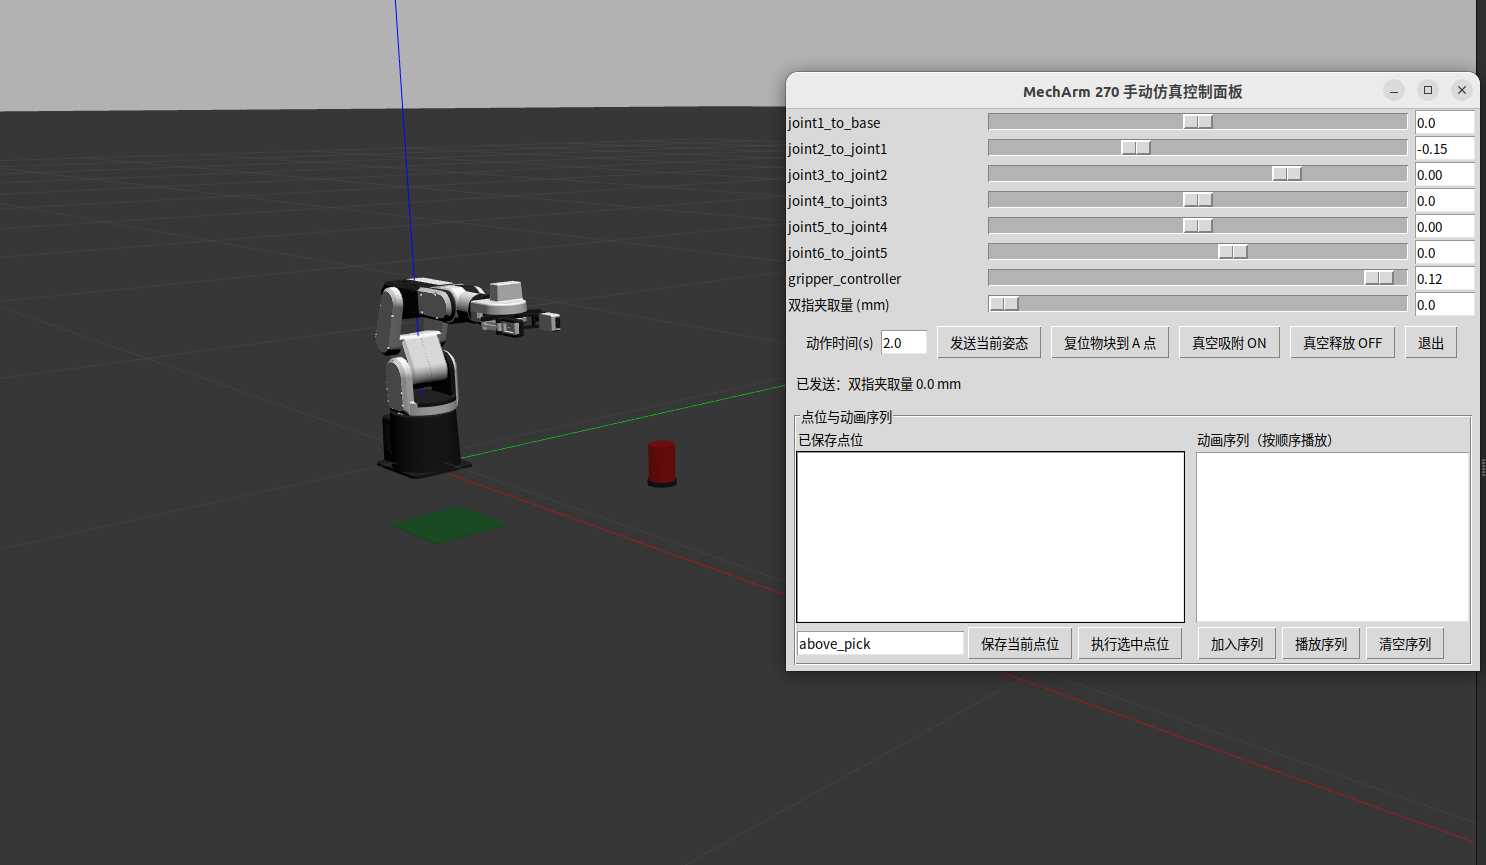
\includegraphics[width=\textwidth]{manual_control_console.png}\end{minipage}
\caption{仿真调试所用的动作序列记录和实际 Gazebo 手动控制台界面。}\label{fig:simmanualzh}\end{figure}

\subsection{实机实现过程}
实机阶段按以下六个步骤完成，流程与仿真状态机保持对应：
\begin{enumerate}
\item \textbf{准备平台与通信。}使用 mechArm 270-Pi 六自由度机械臂和电动夹爪，控制端通过\code{pymycobot}连接\code{/dev/ttyAMA0}，波特率设为 1000000。上电后检查串口、急停、控制库连接状态以及夹爪开合响应，确认控制指令能够被设备接收。
\item \textbf{布置桌面与 A/B 点。}将机械臂固定在准备好的桌面旁，按仿真中的相对位置放置抓取点 A 和放置点 B。检查机械臂基座、桌面边缘和目标区域的距离，保证 SAFE 位姿下末端有足够空间，PICK 和 PLACE 位姿能够垂直接近桌面。
\item \textbf{回到初始位姿。}启动动作程序前让机械臂回到 HOME，确认六个关节处于可运动范围，并将夹爪置于打开状态。先执行一轮低速、空夹爪动作，观察各关节方向、桌面间隙和夹爪朝向，完成实机路径的第一轮确认。
\item \textbf{执行固定点抓取。}程序依次执行 HOME 到 A 点上方 SAFE、下降到 PICK、夹爪 GRIP、抬升回 SAFE。夹爪闭合后观察目标是否保持在夹持中心，机械臂抬升时检查目标是否发生滑落或碰撞。
\item \textbf{搬运、释放与复位。}机械臂沿示教路径移动到 B 点上方 SAFE，下降到 PLACE 位姿，执行 RELEASE，再回到 SAFE 并返回 HOME。释放后的目标位置、末端高度和回程姿态分别作为放置、避障和复位检查项。
\item \textbf{记录现场证据与异常处理。}演示过程中持续观察夹持稳定性、桌面擦碰、放置偏差和串口状态；出现通信异常、目标滑落或姿态异常时，停止连续运动并回到安全姿态。最终 MP4 记录接近、夹持、抬升、搬运、释放和复位画面，仿真 CSV 提供五周期数值结果，二者共同记录控制逻辑从 Gazebo 到实体平台的迁移。
\end{enumerate}
\begin{figure}[H]\centering
\begin{tikzpicture}[node distance=0.33cm,every node/.style={font=\small},s/.style={draw=Navy,rounded corners=2pt,fill=Sky,minimum width=2.25cm,minimum height=0.62cm,align=center},t/.style={s,draw=Teal,fill=Teal!12},a/.style={-Latex,draw=Teal,line width=0.8pt}]
\node[s](r1){串口连接\\状态检查};\node[s,right=of r1](r2){HOME\\夹爪打开};\node[s,right=of r2](r3){A 点\\PICK / GRIP};\node[t,right=of r3](r4){SAFE\\搬运至 B};\node[t,right=of r4](r5){PLACE / RELEASE\\返回 HOME};
\draw[a](r1)--(r2)--(r3)--(r4)--(r5);
\end{tikzpicture}
\caption{实机阶段从设备准备到抓取、搬运、释放和复位的动作链。}\label{fig:realflowzh}
\end{figure}

\section{验证结果}
\subsection{五周期仿真记录}
v2 材料中的两份 CSV 经过 SHA-256 校验且彼此独立。每份包含 116 行：五个完整周期和一行终端摘要。记录中五条\code{cycle\_passed}的最终位置如下。
\begin{table}[H]\centering\small\caption{\code{fixed\_pick\_20260912\_233915.csv}的五周期结果}\begin{tabular}{c c c c c}\toprule 周期 & $x$ (m) & $y$ (m) & $z$ (m) & XY 误差 (m)\\\midrule 1 & 0.2457 & -0.1238 & 0.0200 & 0.0006\\2 & 0.2462 & -0.1241 & 0.0200 & 0.0001\\3 & 0.2459 & -0.1239 & 0.0200 & 0.0005\\4 & 0.2466 & -0.1242 & 0.0200 & 0.0003\\5 & 0.2459 & -0.1239 & 0.0200 & 0.0005\\\midrule \multicolumn{4}{r}{最大 XY 误差} & 0.0006\\\bottomrule\end{tabular}\end{table}
终端摘要给出\code{success\_count=5}、\code{repeat\_count=5}，并采用“5 次中至少成功 4 次”的规则。第二份 CSV 同样为 5/5，最大 XY 误差为 0.0005 m。CSV 中周期号 6 的记录是周期 5 之后写入的终端摘要行，统计周期仍为 5 次。
\subsection{静态检查与异常处理}
验证记录显示 Python 语法、Xacro、URDF 和\code{colcon build}检查均通过。动作开始前，任务节点会检查所有路径点是否位于关节限位内。错误日志记录了最终版本形成过程中遇到的问题：简化夹爪碰撞模型可能将目标弹出，过大的接触包络会造成穿透，启动延迟不足会与控制器激活竞争，重复使用释放点会导致目标重叠。最终通过配置视觉附着模式、缩小用于间隙检查的碰撞几何、延迟启动以及释放后检查 Gazebo 最终位姿解决这些问题。

\section{演示证据}
\subsection{仿真视频}
图~\ref{fig:simvideozh}从\code{simulation\_demo.webm}中选取三帧：第一帧显示机械臂接近工作区域，中间帧显示夹爪携带红色圆柱，最后一帧显示释放后机械臂回到场景初始侧。原始 WebM 随提交包归档。\begin{figure}[H]\centering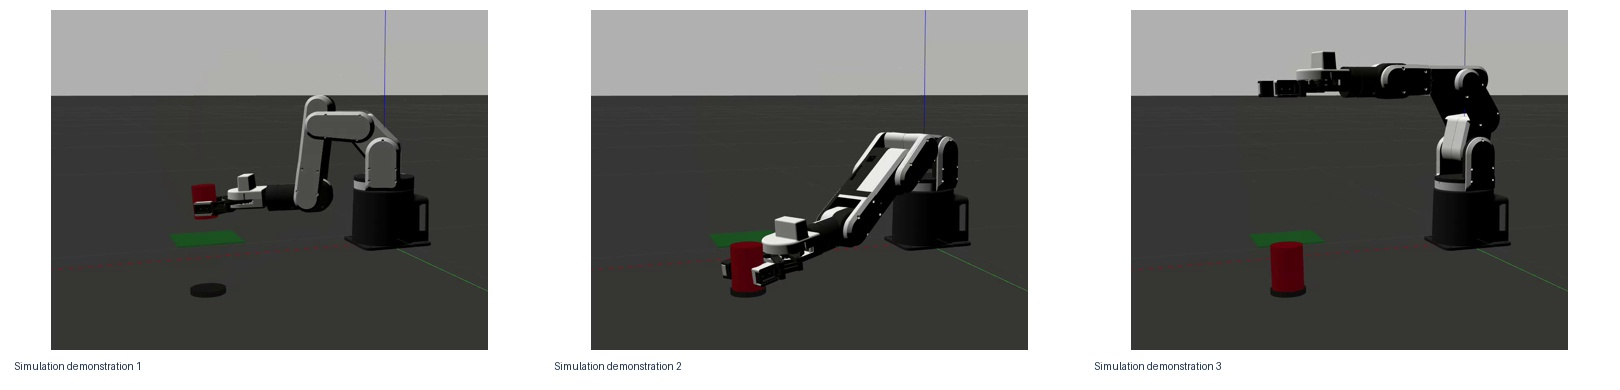
\includegraphics[width=\textwidth]{sim_sequence.jpg}\caption{仿真演示视频中的代表性画面。}\label{fig:simvideozh}\end{figure}
\subsection{实机视频}
图~\ref{fig:realvideozh}概括了提供的竖屏 MP4，画面展示实体机械臂、夹爪、桌面和目标区域，记录了动作迁移到硬件后的运行过程。五周期数值结果见仿真 CSV 记录。\begin{figure}[H]\centering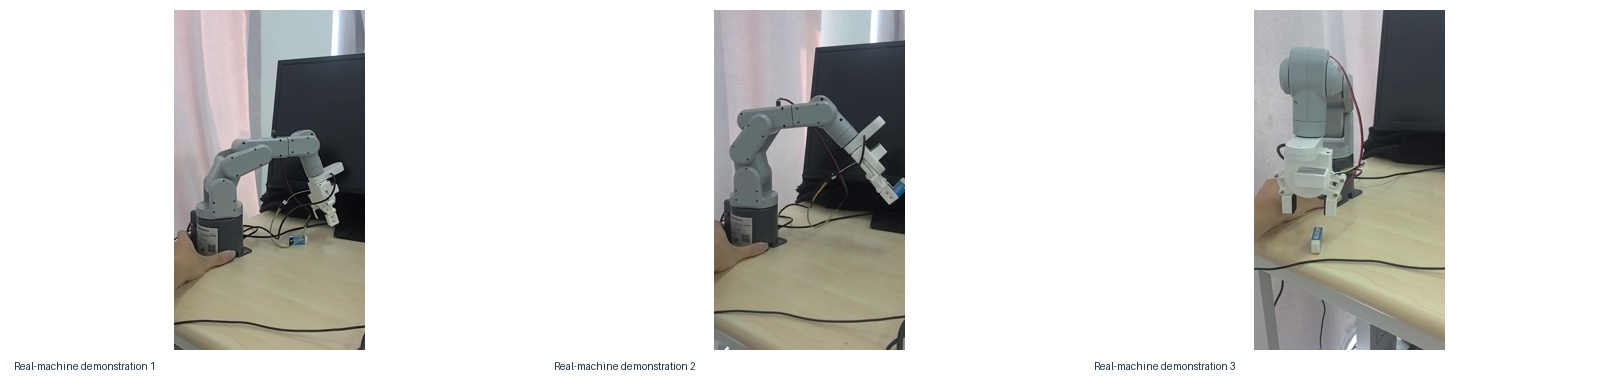
\includegraphics[width=\textwidth]{real_sequence.jpg}\caption{实机演示视频中的代表性画面。}\label{fig:realvideozh}\end{figure}

\section{讨论与总结}
\subsection{实验完成的内容}
最终仿真材料形成了一个完整的定点操作闭环：参数明确、状态机可复现、控制器能够按序启动，目标附着与释放语义清楚，并且有最终位姿检查和持久化 CSV 输出。五周期记录比单张成功截图更能说明重复性，也保留了实际释放坐标。较小的最大 XY 误差说明竖直释放策略与 B 点配置相符。

程序、配置、日志、视频和报告分目录保存。新的使用者可以构建工作空间、运行一个脚本、观察同名状态阶段，并在日志中找到相应记录。这样的组织方式也便于分阶段提交 GitHub，在不下载二进制压缩包的情况下审阅代码和证据。
\subsection{局限与实践体会}
定点任务使用预设 A、B 点，研究重点是路径执行、夹爪动作和放置判定。Gazebo 中的附着机制经过控制，使抓取和释放过程可测量；实体夹爪还会受到柔顺性、摩擦变化、线缆干涉和目标滑移的影响。实验将仿真 CSV 用于定量分析，将实机视频用于说明硬件动作过程。

调试过程表明，最终位姿检查是放置判定的关键。实验记录目标最终 X/Y/Z、释放上方和释放稳定事件，并保留错误日志，从而形成可追踪的动作链路。
\subsection{总结与感悟}
\begin{enumerate}\item 定点操作首先是一个一致性问题：坐标系、示教关节向量、夹爪数值、物体几何和成功阈值必须描述同一个场景。\item 带有明确阶段名称的状态机比无标签的长指令流更容易诊断，CSV 中的阶段名可以定位第一次失败动作。\item 安全运行需要在动作前后都检查：关节限位检查防止非法指令，最终位姿检查防止误报。\item ROS 2 Launch 和参数文件提供了从仿真到实机的接口，控制序列可以保持稳定，而设备和环境参数可以单独替换。\item 完整提交应同时包含源码、日志、视频、LaTeX 源文件和 PDF，并通过校验和、分阶段 Git 提交记录材料的形成过程。\end{enumerate}

\section{提交材料目录}
\begin{table}[H]\centering\small\caption{最终提交目录中的主要文件}\begin{tabularx}{\textwidth}{>{\ttfamily\scriptsize\raggedright\arraybackslash}p{0.46\textwidth}X}\toprule 路径 & 用途\\\midrule \code{src/mecharm\_fixed\_pick\_sim/} & ROS 2 任务节点、Launch、YAML、场景与 URDF/Xacro\\\code{src/mycobot\_description/} & 机器人网格与夹爪资源\\\code{run\_contact\_grasp.sh} & 一条命令启动五周期仿真\\\code{submission\_evidence/results/} & 两份独立五周期 CSV\\\code{submission\_evidence/docs/ERROR\_LOG.md} & 异常情况与修复记录\\\code{submission\_evidence/videos/} & 仿真 WebM 与实机 MP4\\\code{submission\_evidence/SHA256SUMS.txt} & 证据文件校验和\\\code{report/experiment2\_lab\_report.tex} & 英文报告源文件\\\code{report/experiment2\_lab\_report.pdf} & 英文提交 PDF\\\code{report/experiment2\_lab\_report\_zh\_preview.tex} & 中文预览源文件\\\code{report/experiment2\_lab\_report\_zh\_preview.pdf} & 中文预览 PDF\\\bottomrule\end{tabularx}\end{table}
\subsection{GitHub 提交记录}
实验二材料维护在公开仓库\url{https://github.com/9161942-boop/robotics-experiment-2}中，代码、证据、报告和视频按阶段提交：\begin{table}[H]\centering\small\caption{实验二分阶段 GitHub 提交}\begin{tabular}{ll}\toprule 提交 & 内容\\\midrule \code{b21bb71} & ROS 2 程序、Launch 文件与仿真配置\\\code{330ac6a} & 五周期 CSV、错误日志与校验和\\\code{dc85c53} & 英文 LaTeX 报告、PDF 与插图\\\code{b4f67d2} & 仿真和实机演示视频\\\bottomrule\end{tabular}\end{table}
\section*{证据范围说明}\addcontentsline{toc}{section}{证据范围说明}本报告中的仿真结果引用 final v2 压缩包及其中的 CSV、验证记录，编写报告阶段未重新运行仿真。两段视频为用户提供的演示文件，报告依据视频画面说明仿真和实机动作过程。五周期仿真次数由 CSV 支持，实机部分围绕 MP4 中呈现的实体操作展开。
\begin{figure}[H]\centering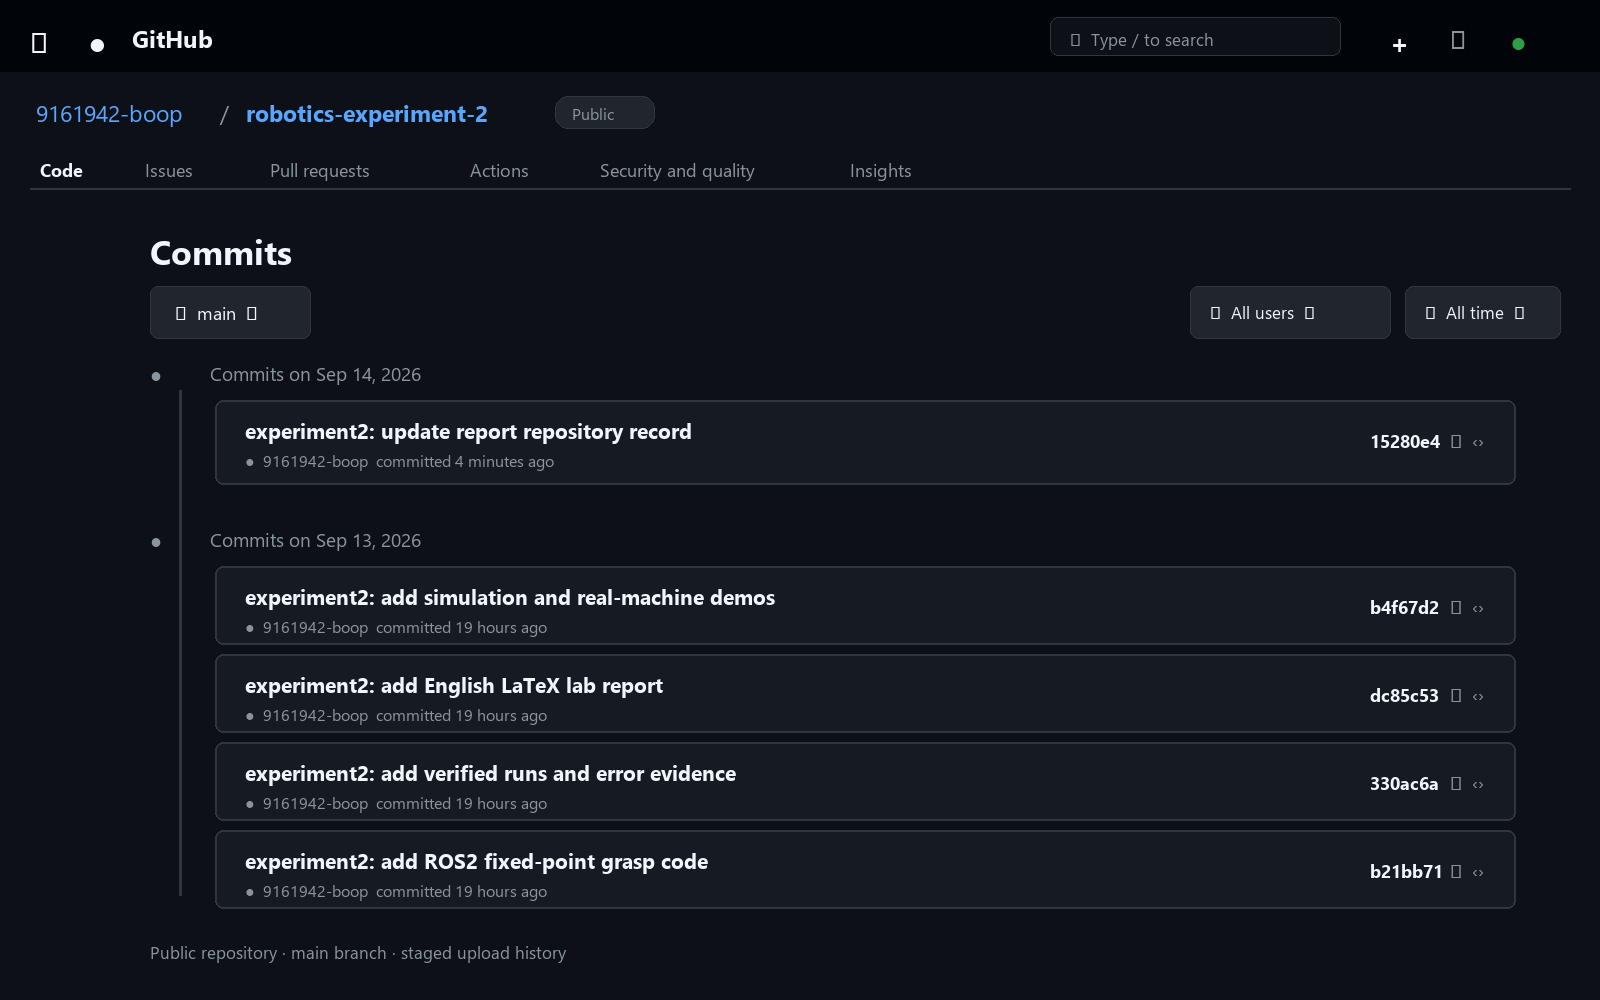
\includegraphics[width=0.55\textwidth]{github_commit_history_exp2.png}\caption{公开实验二仓库的 GitHub 提交历史。}\label{fig:github-history-zh}\end{figure}
\end{document}
